\documentclass{article}
\textheight 23.5cm \textwidth 15.8cm
%\leftskip -1cm
\topmargin -1.5cm \oddsidemargin 0.3cm \evensidemargin -0.3cm
%\documentclass[final]{siamltex}

\usepackage{verbatim}
\usepackage{fancyhdr}
\usepackage{amssymb,ctex}
\usepackage{mathrsfs}
\usepackage{latexsym,amsmath,amssymb,amsfonts,epsfig,graphicx,cite,psfrag}
\usepackage{eepic,color,colordvi,amscd}
\usepackage{enumerate}
\usepackage{booktabs}
\usepackage{graphicx}
\usepackage{float}
\usepackage{multirow}


\title{Numerical Analysis Homework8}
\author{Zhang Jiyao,PB20000204}

\begin{document}
	\maketitle
	
	\section{Introduction}
	利用四阶龙格-库塔方法和各种$\lambda$的值,譬如,$\lambda=5,-5,-10$,数值求解下列初值问题:
	
$$	\left\{ 
	\begin{array}{lc}
		x^{'} = \lambda x+\text{cost}-\lambda \text{sint} \\
		x(0)=0\\
	\end{array}
	\right.$$
	
	并且在区间$[0,5]$上比较数值解和解析解,利用步长$h=0.01$,并考虑$\lambda$对数值的准确性有什么影响。
	
	
	\section{Method}
	 首先我们可以直接求出方程的解析解。通过观察不难发现$x(t)=sint$是方程的一个解,且满足初值条件。
	 
	 下面用四阶龙格-库塔方法求解数值解。
	 $$ x(t+h)=x(t)+\frac{1}{6}(F_1+2F_2+2F_3+F_4)$$
	 其中有
	 $$	
	 \left\{ 
	 \begin{array}{lc}
	 	F_1 = hf(t,x) \\
	    F_2 = hf(t+\frac{1}{2}h,x+\frac{1}{2}F_1) \\
	 	F_3 = hf(t+\frac{1}{2}h,x+\frac{1}{2}F_2) \\
	 	F_4 = hf(t+h,x+F_3) \\
	 \end{array}
	 \right.$$

	
	
	\section{Results}
	
	把数值解和解析解画在一个坐标系内,比较它们的图像
	
		\begin{figure}[H]
		\begin{center}
			
			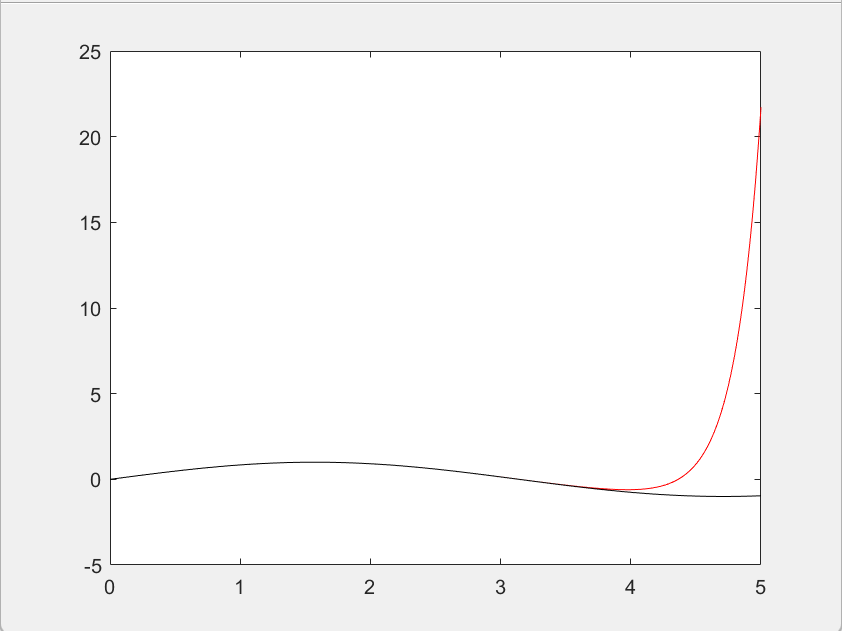
\includegraphics[width=6cm,height=6cm]{5}
			
			\caption{当$\lambda$=5时的图像} \label{5.label}
		\end{center}
	\end{figure}
	
	\begin{figure}[H]
		\begin{center}
			
			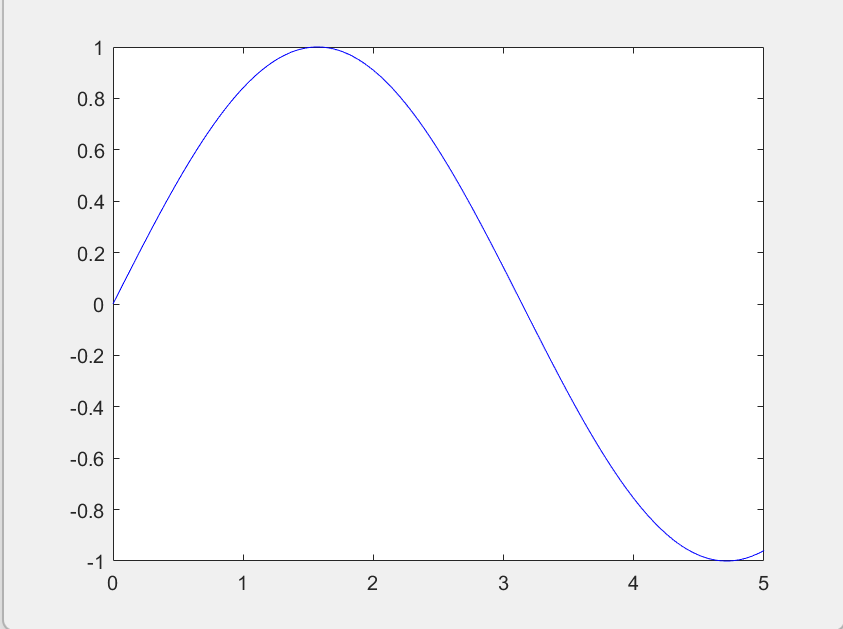
\includegraphics[width=6cm,height=6cm]{-5}
			
			\caption{当$\lambda$=-5时的图像} \label{-5.label}
		\end{center}
	\end{figure}
	
		\begin{figure}[H]
		\begin{center}
			
			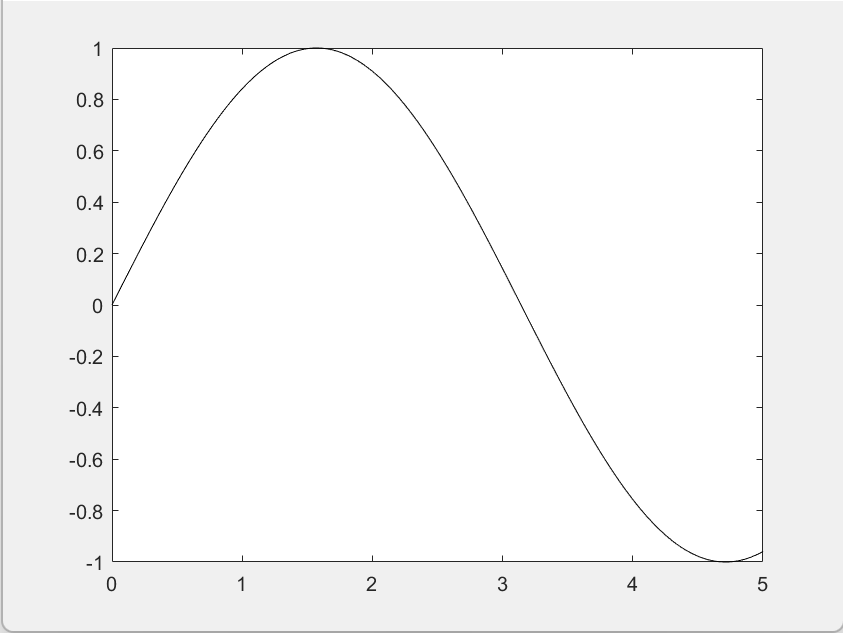
\includegraphics[width=6cm,height=6cm]{-10}
			
			\caption{当$\lambda$=-10时的图像} \label{-10.label}
		\end{center}
	\end{figure}
	
	
	\section{Discussion}
	
	观察结果可以发现,当$\lambda=-5$或$\lambda=-10$时,数值解与解析解结果的差距很小,从图像上是基本看不出来的。通过数值计算发现误差一般在\text{1e-8}量级左右。考虑到四阶龙格-库塔方法的误差是$O(h^5)$,这个结果也是合理的。
	
	当$\lambda=5$时,数值解与解析解差距较大。猜想这可能与$\lambda$的符号有关。因为$\lambda > 0$时,对很大的$x$,总有$x > \text{sinx}$,所以$x'$基本都大于0,因此采用龙格-库塔方法计算带来的误差较大。

	
	
	
	\section{Computer Code}
	\verbatiminput{Runge.m}
	\verbatiminput{main.m}
	
\end{document}